% TODO: cite https://github.com/niklas-heer/speed-comparison
% TODO: gender neutral
\documentclass{beamer}
\usepackage{textcomp}
\usepackage[normalem]{ulem}
\usepackage{listings}

\title{Warum ist Python so cool\textinterrobang}
\author{Lars Quentin}
\date{26.04.2022}
\usetheme[numbering=none]{metropolis}

\begin{document}
\frame{\titlepage}

% TODO: cite
\section{Wie beliebt ist Python?}
{
  \usebackgroundtemplate{
  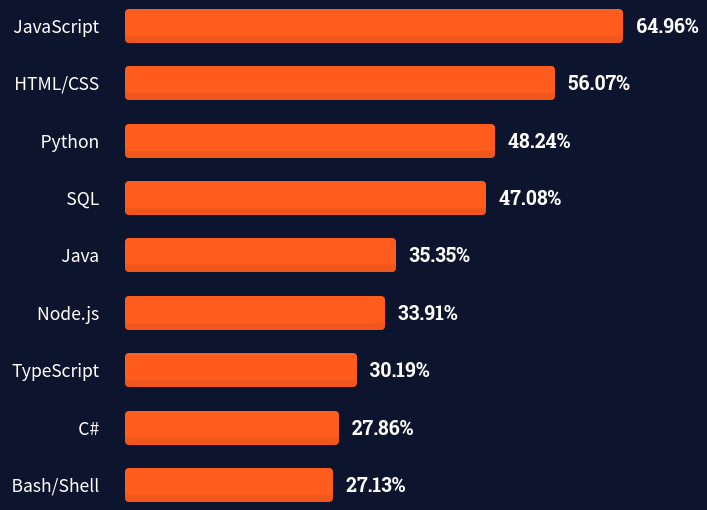
\includegraphics[height=\paperheight,width=\paperwidth]{assets/so1.png}
  }
  \begin{frame}[plain]
  \end{frame}
}
{
  \usebackgroundtemplate{
  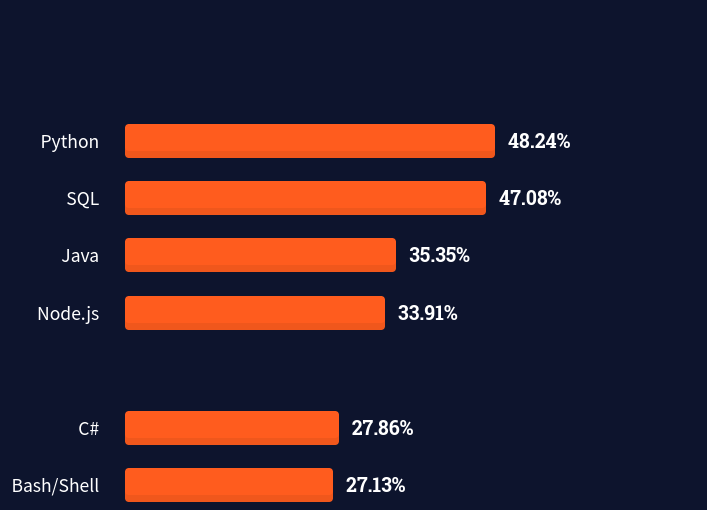
\includegraphics[height=\paperheight,width=\paperwidth]{assets/so2.png}
  }
  \begin{frame}[plain]
  \end{frame}
}
{
  \usebackgroundtemplate{
  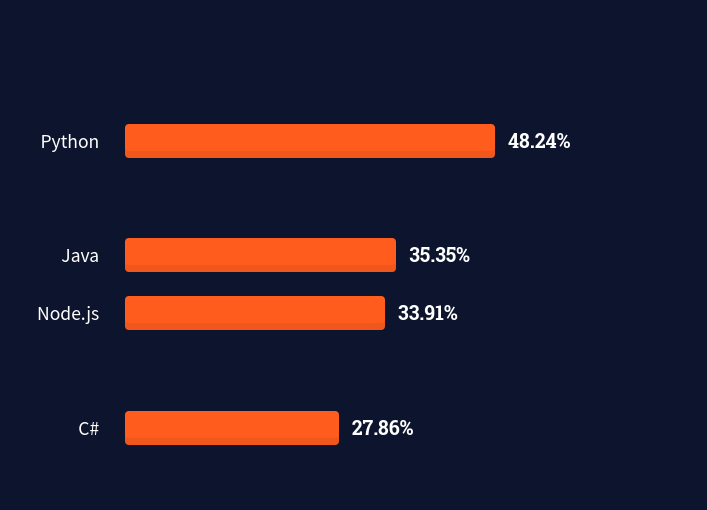
\includegraphics[height=\paperheight,width=\paperwidth]{assets/so3.png}
  }
  \begin{frame}[plain]
  \end{frame}
}

% Warum ich das mache: Dieser Vortrag soll ueber Programmiersprachen gehen.
% Insbesondere soll man hier besondere Konzepte der Sprache vorstellen
\section{Was macht Python so besonders?}
% Erforschen wir mal die Möglichkeiten

\begin{frame}
\begin{center}
{\usebeamerfont*{frametitle} \Huge Plattformexklusivität?}\\~\\
\pause
Nein!
\end{center}
\end{frame}

\begin{frame}
\begin{center}
{\usebeamerfont*{frametitle} \Huge Performance?}
\end{center}
\end{frame}

{
  \usebackgroundtemplate{
  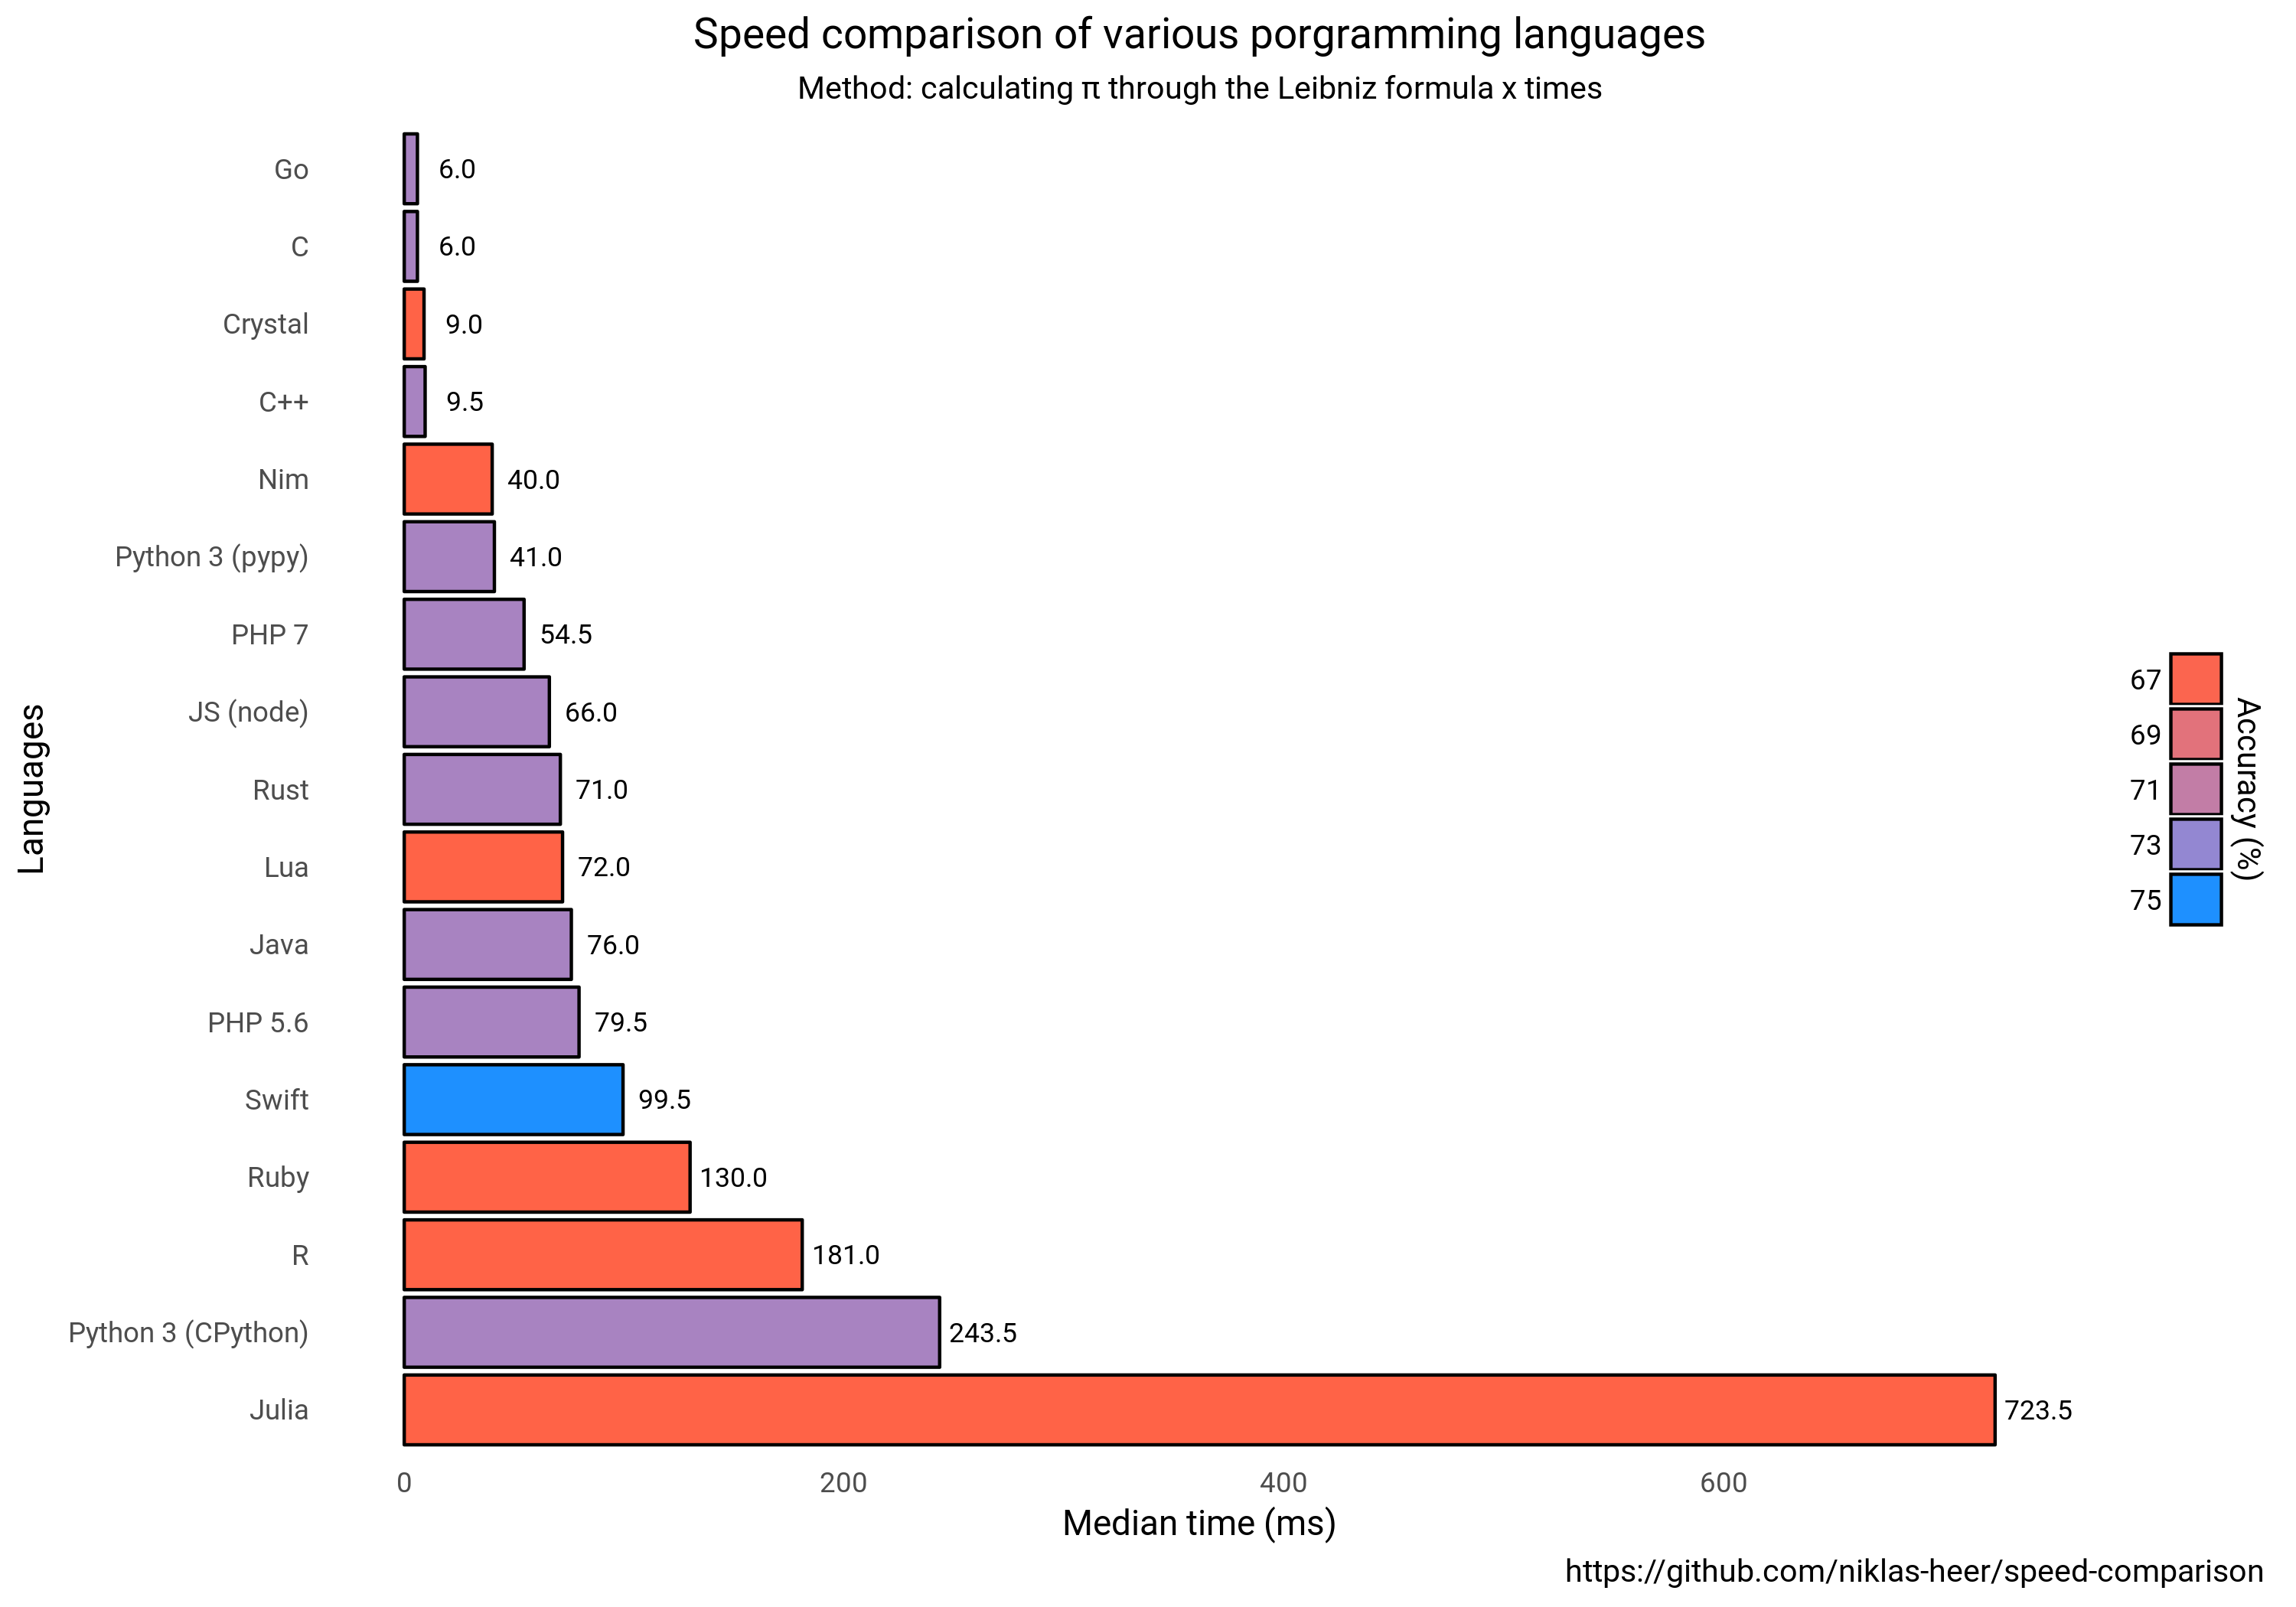
\includegraphics[height=\paperheight,width=\paperwidth]{assets/bench.png}
  }
  \begin{frame}[plain]
  \end{frame}
}

\begin{frame}
\begin{center}
{\usebeamerfont*{frametitle} \Huge Performance?}\\~\\
lol
\end{center}
\end{frame}

\begin{frame}[t]{Was macht Python so besonders?}
Also... was ist es nun?
\pause
\begin{itemize}
\item \sout{Plattformexklusivität}
\pause
\item \sout{Performance}
\pause
\item Revolutionäre Paradigmen?
\end{itemize}
\end{frame}

\begin{frame}[t]{Was macht Python so besonders?}
Also... was ist es nun?
\begin{itemize}
\item \sout{Plattformexklusivität}
\item \sout{Performance}
\item \sout{Revolutionäre Paradigmen?}
\item Einfach bugfreie Programme zu schreiben? % ne das ist haskell :^)
\end{itemize}
\end{frame}

\begin{frame}[t]{Was macht Python so besonders?}
Also... was ist es nun?
\begin{itemize}
\item \sout{Plattformexklusivität}
\item \sout{Performance}
\item \sout{Revolutionäre Paradigmen?}
\item \sout{Einfach bugfreie Programme zu schreiben?}
\item Besondere Sprachfeatures für ML, Webdev, Web3, Embedded...
\end{itemize}
\end{frame}

\begin{frame}[t]{Was macht Python so besonders?}
Also... was ist es nun?
\begin{itemize}
\item \sout{Plattformexklusivität}
\item \sout{Performance}
\item \sout{Revolutionäre Paradigmen?}
\item \sout{Einfach bugfreie Programme zu schreiben?}
\item \sout{Besondere Sprachfeatures für ML, Webdev, Web3, Embedded...}
\end{itemize}
\begin{center}
{~\\~\\\Huge ???????}
\end{center}
\end{frame}

\begin{frame}
\begin{center}
{\usebeamerfont*{frametitle} \Huge Python ist langweilig.}\\~\\
\pause
{\Large Und langweilig ist simpel.}
\end{center}
\end{frame}

\begin{frame}[t]{Aufgabenstellung}
\textbf{Gegeben:}\\
\vspace{0.2cm}
Eine Textdatei mit kommaseparierten Ganzzahlen\\~\\~\\~\\
\textbf{Aufgabe:}
\begin{itemize}
\item Lies die Datei ein
\item Berechne die Summe
\item Berechne die Anzahl der Elemente
\item Gebe den Mittelwert aus
\end{itemize}
\end{frame}

\begin{frame}
\begin{center}
{\usebeamerfont*{frametitle} \Huge Wieso ist Python so gut?}\\~\\
\pause
Vieles!
\end{center}
\end{frame}

\section{Zug\"anglichkeit f\"ur Nicht-Programmierer}

\begin{frame}{Jupyter Notebooks}
\begin{columns}[onlytextwidth,T]
\column{\dimexpr\linewidth-30mm-5mm}
\begin{itemize}
\item Webbasierte Pythonumgebung
\item Interaktiv
\item Grafisch
\item Kostenloses online benutzbar
\begin{itemize}
\item Google Colab
\item Jupyter GWDG
\end{itemize}
\item Open Source, BSD-3 lizensiert
\item Sp\"ater mehr
\end{itemize}
\column{30mm}

\includegraphics[width=30mm]{./assets/jupyter.png}
\end{columns}
\end{frame}

\begin{frame}{Ben\"otigtes Vorwissen}
\begin{center}
\LARGE Was braucht man f\"ur Vorwissen?
\end{center}
\begin{itemize}
\item Typensysteme? Integergr\"o\ss{}en?
\item Kommandozeile?
\item Compiler?
\item Speicher?
\item reinterpret\_cast\textless bool(\_\_stdcall*)(const char*, const char*)\textgreater?
\end{itemize}
\begin{center}
\Large Englischkenntnisse reichen zum lesen.
\end{center}
\end{frame}

\section{Zug\"anglichkeit f\"ur Programmierer}


\end{document}
